% -----------------------------------------------------------------------------
% The MIT License (MIT)
%
% Copyright (c) 2015 Pejman Ghorbanzade
%
% Permission is hereby granted, free of charge, to any person obtaining a copy
% of this software and associated documentation files (the "Software"), to deal
% in the Software without restriction, including without limitation the rights
% to use, copy, modify, merge, publish, distribute, sublicense, and/or sell
% copies of the Software, and to permit persons to whom the Software is
% furnished to do so, subject to the following conditions:
%
% The above copyright notice and this permission notice shall be included in
% all copies or substantial portions of the Software.
%
% THE SOFTWARE IS PROVIDED "AS IS", WITHOUT WARRANTY OF ANY KIND, EXPRESS OR
% IMPLIED, INCLUDING BUT NOT LIMITED TO THE WARRANTIES OF MERCHANTABILITY,
% FITNESS FOR A PARTICULAR PURPOSE AND NONINFRINGEMENT. IN NO EVENT SHALL THE
% AUTHORS OR COPYRIGHT HOLDERS BE LIABLE FOR ANY CLAIM, DAMAGES OR OTHER
% LIABILITY, WHETHER IN AN ACTION OF CONTRACT, TORT OR OTHERWISE, ARISING FROM,
% OUT OF OR IN CONNECTION WITH THE SOFTWARE OR THE USE OR OTHER DEALINGS IN
% THE SOFTWARE.
% -----------------------------------------------------------------------------

\def \topDirectory {../..}

\documentclass[10pt, compress]{beamer}

\usepackage{\topDirectory/template/style/directives}
% -----------------------------------------------------------------------------
% The MIT License (MIT)
%
% Copyright (c) 2015 Pejman Ghorbanzade
%
% Permission is hereby granted, free of charge, to any person obtaining a copy
% of this software and associated documentation files (the "Software"), to deal
% in the Software without restriction, including without limitation the rights
% to use, copy, modify, merge, publish, distribute, sublicense, and/or sell
% copies of the Software, and to permit persons to whom the Software is
% furnished to do so, subject to the following conditions:
%
% The above copyright notice and this permission notice shall be included in
% all copies or substantial portions of the Software.
%
% THE SOFTWARE IS PROVIDED "AS IS", WITHOUT WARRANTY OF ANY KIND, EXPRESS OR
% IMPLIED, INCLUDING BUT NOT LIMITED TO THE WARRANTIES OF MERCHANTABILITY,
% FITNESS FOR A PARTICULAR PURPOSE AND NONINFRINGEMENT. IN NO EVENT SHALL THE
% AUTHORS OR COPYRIGHT HOLDERS BE LIABLE FOR ANY CLAIM, DAMAGES OR OTHER
% LIABILITY, WHETHER IN AN ACTION OF CONTRACT, TORT OR OTHERWISE, ARISING FROM,
% OUT OF OR IN CONNECTION WITH THE SOFTWARE OR THE USE OR OTHER DEALINGS IN
% THE SOFTWARE.
% -----------------------------------------------------------------------------

\course{id}{CS114}
\course{name}{Introduction to Java}
\course{venue}{Mon/Wed, 5:30 PM - 6:45 PM}
\course{semester}{Fall 2015}
\course{department}{Department of Computer Science}
\course{university}{University of Massachusetts Boston}

\instructor{name}{Pejman Ghorbanzade}
\instructor{title}{}
\instructor{position}{Student Instructor}
\instructor{email}{pejman@cs.umb.edu}
\instructor{phone}{617-287-6419}
\instructor{office}{S-3-124B}
\instructor{office-hours}{Mon/Wed 16:00-17:30}
\instructor{address}{University of Massachusetts Boston, 100 Morrissey Blvd., Boston, MA}

\usepackage{\topDirectory/template/style/beamerthemeUmassLecture}
\doc{number}{2}
%\setbeamertemplate{footline}[text line]{}

\begin{document}
\prepareCover

\section{Course Administration}

\begin{frame}[fragile]
	\frametitle{Course Administration}
	\begin{itemize}
		\item[] Create user accounts at \href{http://www.ghorbanzade.com}{Course Website}.
		\item[] Midterm exam to be held October 21st, 2015.
	\end{itemize}
\end{frame}

\begin{frame}[fragile]
	\frametitle{Course Administration}
	\begin{block}{Overview}
		\begin{itemize}
			\item[] Computer Hardwares
			\item[] Computer Programming
			\item[] Programming Languages
		\end{itemize}
	\end{block}
\end{frame}

\section{Computer Hardware}

\begin{frame}
	\frametitle{Computer Hardware}
	\begin{block}{Key Components}
		\begin{itemize}
			\item[] Central Processing Unit (CPU)
			\item[] Input Output (I/O) Devices
			\item[] Memory
		\end{itemize}
	\end{block}
\end{frame}

\begin{frame}
	\frametitle{Computer Hardware}
	\begin{block}{Key Design Challenges}
		\begin{itemize}
			\item[] Making Processing Units as small and powerful as possible
			\item[] Making Input Output (I/O) Devices as heterogenous as possible
			\item[] Making Memory as abundant as possible
		\end{itemize}
	\end{block}
\end{frame}

\begin{frame}
	\frametitle{Computer Hardware}
	\begin{block}{Basic Operation Procedure}
		\begin{enumerate}
			\item[] Instructions read either from I/O devices or from memory
			\item[] Each statement processed in processor
			\item[] Output passed either to I/O devices or to memory
		\end{enumerate}
	\end{block}
\end{frame}

\begin{frame}
	\frametitle{Computer Hardware}
	\begin{block}{Mircroprocessor Internal Architecture}
		Key Components
		\begin{enumerate}
			\item[] Arithmetic Logic Unit (ALU)
			\item[] Control Logic Station
			\item[] Status Registers
		\end{enumerate}
	\end{block}
\end{frame}

\begin{frame}
	\frametitle{Computer Hardware}
	\begin{block}{Nature of Information}
		Analog vs. Digital Signals

		2-Base Numeral Systems
		\begin{enumerate}
			\item[] Relation to Digital Electronic Circuitry
			\item[] Reliable Distingushing Property
		\end{enumerate}
	\end{block}
\end{frame}

\section{Computer Programming}

\begin{frame}[fragile]
	\frametitle{Computer Programming}
	\begin{block}{Philosophy}
		\begin{columns}
			\begin{column}{0.4\textwidth}
			\begin{itemize}
				\item[] Strong Points
				\begin{itemize}
					\item[] Fast computing
					\item[] No fatigue
				\end{itemize}
				\item[] Weak Points
				\begin{itemize}
					\item[] Hard to Teach
					\item[] No Innovation
				\end{itemize}
			\end{itemize}
			\end{column}
			\begin{column}{0.6\textwidth}
			\begin{figure}[H]\centering
				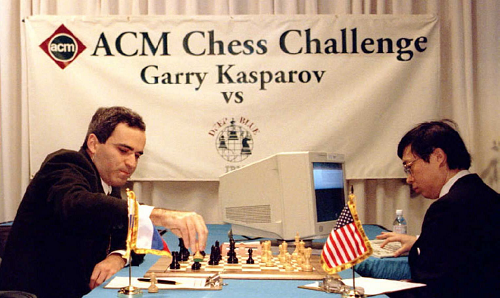
\includegraphics[width=\textwidth]{\topDirectory/template/images/chess.png}
			\end{figure}
			\end{column}
		\end{columns}
	\end{block}
\end{frame}

\begin{frame}[fragile]
	\frametitle{Computer Programming}
	\begin{block}{Computers are good at}
		\begin{itemize}
			\item[] Repetitive simple but tedious computations
			\item[] One-time long and complex computations
		\end{itemize}
	\end{block}
	\begin{block}{Motivation}
		To harvest computers power for solving everyday problems
	\end{block}
\end{frame}

\begin{frame}[fragile]
	\frametitle{Computer Programming}
	\begin{block}{Conflicts}
			\begin{itemize}
				\item[] Computers speak in zeros and ones.
				\item[] Humans speak in prose and verse.
			\end{itemize}
	\end{block}
	\begin{quote}
		Programming languages are efforts to develop a common language easy-to-understand for both.
	\end{quote}
\end{frame}

\begin{frame}[fragile]
	\frametitle{Computer Programming}
	\begin{block}{It's all about thinking}
		\begin{quote}
		``Instead of imagining that our main task is to instruct a computer what to do, let us concentrate rather on explaining to human beings what we want a computer to do.''
		\begin{flushright}
		- Donald Knuth
		\end{flushright}
		\end{quote}
	\end{block}
\end{frame}

\section{Programming Languages}

\begin{frame}[fragile]
	\frametitle{Programming Languages}
	\begin{block}{Classification}
		\begin{columns}
			\begin{column}{0.5\textwidth}
			\begin{itemize}
				\item[] By level of abstraction
				\begin{itemize}
					\item[] Low-level languages
					\item[] High-level languages
					\item[] Very-high-level languages
					\item[]
				\end{itemize}
			\end{itemize}
			\end{column}
			\begin{column}{0.5\textwidth}
			\begin{itemize}
				\item[] By method of execution
				\begin{itemize}
					\item[] Machine Code
					\item[] Assembler
					\item[] Compiler
					\item[] Interpreter
				\end{itemize}
			\end{itemize}
			\end{column}
		\end{columns}
	\end{block}
\end{frame}

\begin{frame}[fragile]
	\frametitle{Programming Languages}
	\begin{block}{A Closer Look}
		\begin{figure}\centering
			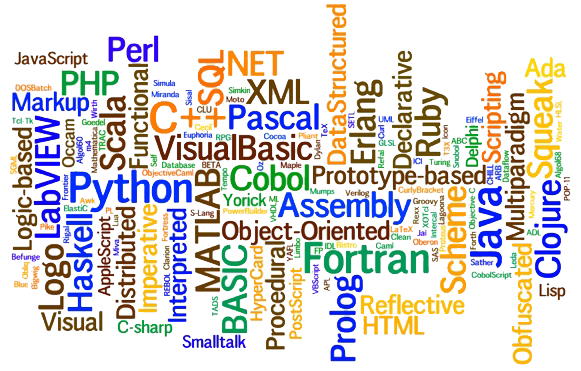
\includegraphics[width=\textwidth]{\topDirectory/template/images/languages.png}
		\end{figure}
	\end{block}
\end{frame}

\begin{frame}[fragile]
	\frametitle{Programming Languages}
	\begin{block}{A Closer Look}
		Let's taste some code!
		\begin{columns}
			\begin{column}{0.5\textwidth}
			\begin{itemize}
				\item[] Machine Language
				\item[] Assembly
				\item[] C
				\item[] C++
				\item[] Python
			\end{itemize}
			\end{column}
			\begin{column}{0.5\textwidth}
			\begin{itemize}
				\item[] Perl
				\item[] Ruby
				\item[] Matlab
				\item[] LabVIEW
				\item[] Scratch
			\end{itemize}
			\end{column}
		\end{columns}
	\end{block}
\end{frame}

\plain{}{Keep Calm\\and\\Love Programming}

\end{document}
